\chapter{Siła opresji}
\begin{figure}[h]
\centering
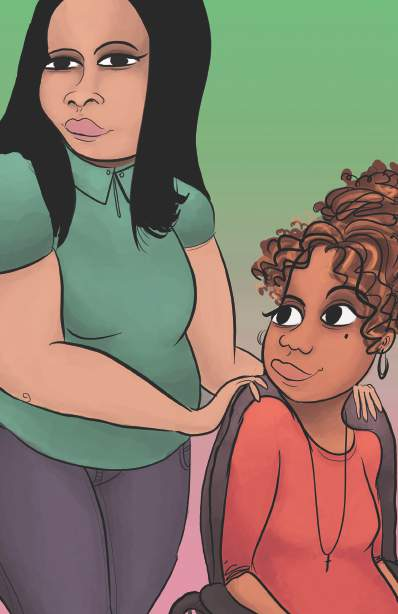
\includegraphics[height=12cm]{TeX_files/2-0.png}
\caption{Artysta: Mohammed Fayaz}
\label{2-0}
\end{figure}


\newpage
\begin{figure}[h]
\centering
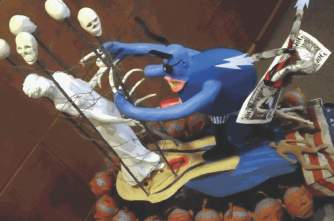
\includegraphics[width=16cm]{TeX_files/2-1.png}
\caption{Artysta: JW Arndt}
\label{2-1}
\end{figure}

\noindent\textcolor{ProcessBlue}{\textbf{\Large{W jaki sposób opresja wpływa na twoje uczucia?}}}\\
\large{\textbf{Oto emocje, które zidentyfikowaliśmy:}}
\begin{multicols}{3}
\begin{itemize}
\item[$\square$]{Rozzłoszczony}
\item[$\square$]{Niespokojny}
\item[$\square$]{Emocjonalnie wyczerpany}
\item[$\square$]{Rozwścieczony}
\item[$\square$]{Smutny}
\item[$\square$]{Zrozpaczony}
\item[$\square$]{Zasmucony}
\item[$\square$]{Bezradny}
\item[$\square$]{Bezsilny}
\item[$\square$]{Zawstydzony}
\item[$\square$]{Zmartwiony}
\item[$\square$]{Zakłopotany}
\item[$\square$]{Sfrustrowany}
\item[$\square$]{Bezwartościowy}
\item[$\square$]{Zaniepokojony}
\item[$\square$]{Zdradzony}
\item[$\square$]{Zmieszany}
\item[$\square$]{Izolujący się}
\item[$\square$]{Fizycznie wyczerpany}
\item[$\square$]{Buntowniczy}
\item[$\square$]{Odczuwający pustkę}
\item[$\square$]{Upokorzony}
\item[$\square$]{Nieufny}
\item[$\square$]{Zdenerwowany}
\item[$\square$]{Przygnębiony}
\item[$\square$]{Zdezorientowany}
\item[$\square$]{Defensywny}
\item[$\square$]{Onurzony}
\item[$\square$]{Niecierpliwy}
\item[$\square$]{Wrogi}
\item[$\square$]{Spięty}
\item[$\square$]{Zraniony}
\item[$\square$]{Rozczarowany}
\item[$\square$]{Wyobcowany}
\end{itemize}
\end{multicols}


\newpage
\noindent
\textcolor{ProcessBlue}{\textbf{\Large{Jakie inne emocje odczuwasz, kiedy doświadczasz opresji?}}}\\\\
\noindent\rule{\textwidth}{1pt}\\
\noindent\rule{\textwidth}{1pt}\\
\noindent\rule{\textwidth}{1pt}\\
\noindent\rule{\textwidth}{1pt}\\
\noindent\rule{\textwidth}{1pt}\\
\noindent\rule{\textwidth}{1pt}\\
\noindent\rule{\textwidth}{1pt}\\
\noindent\rule{\textwidth}{1pt}\\\\

\noindent\textcolor{ProcessBlue}{\textbf{\Large{W jaki sposób opresja wpływa na twoje zachowanie?}}}\\
\textbf{\large{Oto sposoby, które opisaliśmy:}}
\begin{multicols}{2}
\begin{itemize}
\item[$\square$]{Ukrywam się.}
\item[$\square$]{Przejadam się.}
\item[$\square$]{Nie jestem w stanie jeść.}
\item[$\square$]{Uciekam w sen.}
\item[$\square$]{Cierpię na bezsenność.}
\item[$\square$]{Atakuję.}
\item[$\square$]{Potrzebuję fizycznego dystansu od ludzi.}
\item[$\square$]{Zachowuję się jak szalony.}
\item[$\square$]{Staję się uległy.}
\item[$\square$]{Staję się brutalny.}
\item[$\square$]{Zastygam w bezruchu.}
\item[$\square$]{Przestaję rozmawiać.}
\item[$\square$]{Jąkam się.}
\item[$\square$]{Załamuję się emocjonalnie.}
\item[$\square$]{Przestaję o siebie dbać.}
\item[$\square$]{Mam koszmary.}
\item[$\square$]{Jestem biernie agresywny.}
\item[$\square$]{Chcę się odegrać.}
\item[$\square$]{Boję się przyszłości.}
\item[$\square$]{Czuję, że moje życie się rozpada.}
\item[$\square$]{Izoluję się.}
\item[$\square$]{Stosuję uniki.}
\item[$\square$]{Wycofuję się.}
\item[$\square$]{Uciekam w świat wyobraźni.}
\item[$\square$]{Trzęsę się.}
\item[$\square$]{Zastygam w bezruchu.}
\end{itemize}
\end{multicols}


\newpage
\noindent
\textcolor{ProcessBlue}{\textbf{\Large{W jaki sposób opresja wpływa na to, jak się zachowujesz?}}}\\\\
\noindent\rule{\textwidth}{1pt}\\
\noindent\rule{\textwidth}{1pt}\\
\noindent\rule{\textwidth}{1pt}\\
\noindent\rule{\textwidth}{1pt}\\
\noindent\rule{\textwidth}{1pt}\\
\noindent\rule{\textwidth}{1pt}\\
\noindent\rule{\textwidth}{1pt}\\
\noindent\rule{\textwidth}{1pt}\\\\

\noindent\textcolor{ProcessBlue}{\textbf{\Large{W jaki sposób opresja sprawia, że jest ci źle?}}}\\
\textbf{\large{Oto sposoby, które zidentyfikowaliśmy:}}
\begin{multicols}{2}
\begin{itemize}
\item[$\square$]{Próbowałam/Próbowałem popełnić samobójstwo.}
\item[$\square$]{Mam myśli samobójcze.}
\item[$\square$]{Mam ataki paniki.}
\item[$\square$]{Mam bóle głowy.}
\item[$\square$]{Mam bóle brzucha.}
\item[$\square$]{Doświadczam depresji.}
\item[$\square$]{Odzuwam niepokój i paranoję.}
\item[$\square$]{Mam nieustanne negatywne mysli.}
\item[$\square$]{Odczuwam zawroty głowy.}
\item[$\square$]{Mam zaburzenia odżywiania.}
\item[$\square$]{Nadużywam alkoholu i/lub narkotyków.}
\item[$\square$]{Mam koszmary.}
\item[$\square$]{Doświadczam zakłócenia snu.}
\item[$\square$]{Mam wrzody.}
\item[$\square$]{Nasilają się wszelkie moje symptomy.}
\item[$\square$]{Fear and paranoia of healthcare}
\item[$\square$]{Dokonuję samookaleczeń.}
\item[$\square$]{Nienawiść do siebie.}
\item[$\square$]{Cierpię na bezsenność.}
\item[$\square$]{Dochodzi do epizodów maniakalnych.}
\item[$\square$]{Doświadczam PTSD.}
\item[$\square$]{Mam ,,urojenia''.}
\item[$\square$]{Mam ,,psychozy''.}
\item[$\square$]{Izoluję się.}
\item[$\square$]{Mam wysypkę.}
\item[$\square$]{Mam kompulsywne zachowania.}
\item[$\square$]{Wykazuję obsesyjne zachowania.}
\item[$\square$]{Mam depresję.}
\end{itemize}
\end{multicols}


\newpage
\noindent
\textcolor{ProcessBlue}{\textbf{\Large{W jaki sposób opresja manifestuje się w twoim ciele i~umyśle?}}}\\\\
\noindent\rule{\textwidth}{1pt}\\
\noindent\rule{\textwidth}{1pt}\\
\noindent\rule{\textwidth}{1pt}\\
\noindent\rule{\textwidth}{1pt}\\
\noindent\rule{\textwidth}{1pt}\\
\noindent\rule{\textwidth}{1pt}\\
\noindent\rule{\textwidth}{1pt}\\
\noindent\rule{\textwidth}{1pt}\\\\

\noindent\textcolor{ProcessBlue}{\textbf{\Large{W jaki sposób mikroagresja zagraża twojemu dobremu samopoczuciu?}}}\\
\textbf{\large{Oto, jak niektórzy z nas opisali to doświadczenie:}}
\begin{multicols}{2}
\begin{itemize}
\item[$\square$]{Wstyd za siebie.}
\item[$\square$]{Przyśpieszony puls.}
\item[$\square$]{Staję się naprawdę zdenerwowany lub wzburzony.}
\item[$\square$]{Wykazuję nadmierną agresję.}
\item[$\square$]{Staję się brutalny.}
\item[$\square$]{Dokonuję samookaleczeń.}
\item[$\square$]{Jestem przestraszony.}
\item[$\square$]{Jestem sfrustrowany.}
\item[$\square$]{Jest mi smutno i powraca fala wspomnień.}
\item[$\square$]{Rozpraszam się i tracę skupienie.}
\item[$\square$]{Nie radzę sobie.}
\item[$\square$]{Odczuwam niepokój.}
\item[$\square$]{Natrętne myśli.}
\item[$\square$]{Dzwonienie w uszach.}
\item[$\square$]{Uderzenia gorąca.}
\item[$\square$]{Flashbacki.}
\item[$\square$]{Wzburzenie.}
\item[$\square$]{Lęk.}
\item[$\square$]{Smutek.}
\item[$\square$]{Niepokój.}
\item[$\square$]{Nadmierna czujność.}
\item[$\square$]{Przyśpieszenie pulsu.}
\item[$\square$]{Złość.}
\item[$\square$]{Dezorientacja.}
\item[$\square$]{Zawroty głowy.}
\item[$\square$]{Mdłości.}
\item[$\square$]{Drżenie.}
\end{itemize}
\end{multicols}


\newpage
\noindent
\textcolor{ProcessBlue}{\textbf{\Large{W jakie inne sposoby mikroagresja zagraża twojemu dobremu samopoczuciu?}}}\\
\noindent\rule{\textwidth}{1pt}\\
\noindent\rule{\textwidth}{1pt}\\
\noindent\rule{\textwidth}{1pt}\\
\noindent\rule{\textwidth}{1pt}\\
\noindent\rule{\textwidth}{1pt}\\
\noindent\rule{\textwidth}{1pt}\\
\noindent\rule{\textwidth}{1pt}\\
\noindent\rule{\textwidth}{1pt}\\
\noindent\rule{\textwidth}{1pt}\\\\

\noindent\textcolor{ProcessBlue}{\textbf{\Large{W jaki sposób opresja wpływa na to, jak widzisz siebie?}}}\\
\textbf{\large{Oto sposoby, które zidentyfikowaliśmy:}}
\begin{multicols}{2}
\begin{itemize}
\item[$\square$]{Jest mi ze sobą źle.}
\item[$\square$]{Czuję, że lepiej, aby mnie tu nie było.}
\item[$\square$]{Staję się egocentryczna/egocentryczny.}
\item[$\square$]{Złoszczę się na siebie.}
\item[$\square$]{Nienawidzę siebie.}
\item[$\square$]{Wpadam w próbę dopasowania się do ideału samego/samej siebie, zamiast uczciwie być sobą.}
\item[$\square$]{Kwestionuję swoją zdolność do osiągania celów.}
\item[$\square$]{Kwestionuję to, że kiedykolwiek osiągnę szczęście.}
\item[$\square$]{Obawiam się, że nie jestem ,,wart''/ ,,warta'' bycia kochaną/kochanym.}
\item[$\square$]{Czuję się podkopywana/podkopywany.}
\item[$\square$]{Zastanawiam się, czy po prostu wszystko robię źle, co szybko prowadzi do gorszego samopoczucia.}
\item[$\square$]{Czuję się zdystansowany od siebie, rozbity i niepewny przyszłości.}
\item[$\square$]{Czuję się nieskupiony i wycofany.}
\item[$\square$]{Obwiniam siebie.}
\item[$\square$]{Mam myśli, że ,,trzeba było tego robić!”.}
\item[$\square$]{Ciężko jest mi czuć się silną/silnym i skuteczną/skutecznym w świecie.}
\item[$\square$]{Za każdym razem, gdy to się dzieje, muszę na nowo nawiązywać relację ze sobą.}
\item[$\square$]{Wstyd i nienawiść towarzyszą mi, bardzo ciężko jest je zostawić za sobą.}
\item[$\square$]{Wstyd i nienawiść towarzyszą mi, bardzo ciężko jest je zostawić za sobą.}
\item[$\square$]{Obserwuję, jak mój umysł wiruje od złości, winy i frustracji.}
\item[$\square$]{Wątpię w siebie.}
\item[$\square$]{Mam obniżoną pewność siebie w odniesieniu do moich możliwości wchodzenia w interakcje z innymi o oceniania innych.}
\item[$\square$]{Czuję się zdesperowany i bezwartościowy, analizując dawne krzywdy.}
\item[$\square$]{Nie umiem radzić sobie z myślami o przyszłych krzywdach.}
\item[$\square$]{Mam przełączenie i ,,zmiany'', które mogą wyglądać jak wahania nastroju, lecz nimi nie są.}
\item[$\square$]{Często zmagam się z nienawiścią do siebie i wstydem.}
\item[$\square$]{Czuję się ,,mniej niż'' i gorszy od swoich równieśników.}
\item[$\square$]{Często czuję się wyobcowana/wyobcowany od siebie.}
\end{itemize}
\end{multicols}

\begin{figure}[h]
\centering
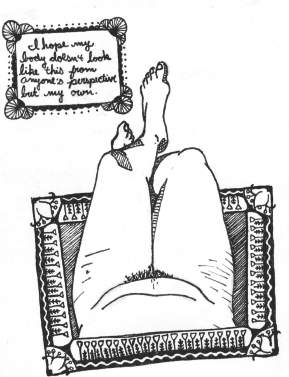
\includegraphics[height=16cm]{TeX_files/2-2.png}
\caption{Artysta: Jodi Bentivegna}
\label{2-2}
\end{figure}

\newpage
\noindent
\textcolor{ProcessBlue}{\textbf{\Large{W jaki sposób opresja wpływa na to, jak postrzegasz siebie?}}}\\
\noindent\rule{\textwidth}{1pt}\\
\noindent\rule{\textwidth}{1pt}\\
\noindent\rule{\textwidth}{1pt}\\
\noindent\rule{\textwidth}{1pt}\\
\noindent\rule{\textwidth}{1pt}\\
\noindent\rule{\textwidth}{1pt}\\
\noindent\rule{\textwidth}{1pt}\\
\noindent\rule{\textwidth}{1pt}\\\\

\noindent\textcolor{ProcessBlue}{\textbf{\Large{Jakie są społeczne konsekwencje opresji?}}}\\
\textbf{\large{Wpływa ona na nasze relacje z przyjaciółmi, rodziną i partnerami w następujący sposob:}}
\begin{multicols}{2}
\begin{itemize}
\item[$\square$]{Nie mam przyjaciół.}
\item[$\square$]{Moja rodzina nie rozmawia ze mną.}
\item[$\square$]{Izoluję się.}
\item[$\square$]{W złości atakuję swoją rodzinę i przyjaciół.}
\item[$\square$]{Kiedy zacząłem/zaczęłam być otwara/otwarty, moja rodzina zaczęła traktować mnie jak czarny charakter i mówić mi, że jestem samolubna/samolubny.}
\item[$\square$]{Przyjaciele, którzy nie rozumieją, czym jest opresja, nie znają mnie całkowicie, ponieważ nie widzą tego kontekstu.}
\item[$\square$]{Muszę zmagać się z moimi wewnętrznie uwarunkowanymi reakcjami na seks, które sygnalizują ,,uwaga, jesteś wykorzystywana/wykorzystywany'', tak abym mogła/mógł doświadczyć go w inny sposób (to znaczy pozytywny) lub nawet w ogóle go doświadczyć i nie być przejrzana/przejrzany.}
\item[$\square$]{Żywię urazę.}
\item[$\square$]{To sprawia, że jestem ostrożny.}
\item[$\square$]{Mam trudności w ufaniu sobie lub innym.}
\item[$\square$]{To sprawia, że komunikacja jest bardzo wymagająca.}
\item[$\square$]{To sprawia, że jest mi trudno czuć się komfortowo w sytuacjach w grupie.}
\item[$\square$]{Mam trudności w utrzymywaniu kontaktów społecznych i odczuwaniu bezpieczeństwa przy wyrażaniu emocji wśród innych.}
\item[$\square$]{Czasami zachowuję się, jakbym był/była poddawana/poddawany opresji w relacjach, nawet, jeśli nie jestem.}
\end{itemize}
\end{multicols}


\newpage
\noindent
\textbf{\large{Wpływa ona na nasze szere środowisko w następujący sposob:}}
\begin{multicols}{2}
\begin{itemize}
\item[$\square$]{Izoluję się.}
\item[$\square$]{Jestem wyobcowany od wszystkich z wyjątkiem swoich rówieśników.}
\item[$\square$]{I still have a hard time believing I will be accepted and trusted by people.}
\item[$\square$]{My circles are somewhat small and I don’t have relationships from when I was younger.}
\item[$\square$]{Sometimes I realize it takes me a long time to accomplish what other folks might see as simple communications.}
\item[$\square$]{I limit how much I connect with people around me in public places and in the community because of my lack of confidence and fear of not being accepted or respected}
\item[$\square$]{Feeling that I cannot expect to feel safe in the broader world leads me to being timid and half present}
\item[$\square$]{I don’t feel a sense of belonging to my broader community}
\item[$\square$]{My interactions are limited and superficial. I put on a happy face and stay in line}
\item[$\square$]{I can’t let anyone know my struggles}
\item[$\square$]{I am utterly convinced that the wider community despises me and wants nothing to do with me}
\item[$\square$]{I feel I have nothing to offer, or give, or do}
\item[$\square$]{It makes it difficult to find a place and a way to contribute meaningfully to the community}
\end{itemize}
\end{multicols}

\noindent
\textcolor{ProcessBlue}{\textbf{\Large{Jakich innych społecznych konsekwencji opresji doświadczas?}}}\\
\noindent\rule{\textwidth}{1pt}\\
\noindent\rule{\textwidth}{1pt}\\
\noindent\rule{\textwidth}{1pt}\\
\noindent\rule{\textwidth}{1pt}\\
\noindent\rule{\textwidth}{1pt}\\
\noindent\rule{\textwidth}{1pt}\\
\noindent\rule{\textwidth}{1pt}\\
\noindent\rule{\textwidth}{1pt}\\
\noindent\rule{\textwidth}{1pt}\\\\


\newpage
\begin{figure}[h]
\centering
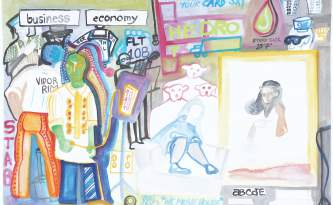
\includegraphics[width=16cm]{TeX_files/2-3.png}
\caption{Artist: Eddy Falconer}
\label{2-2}
\end{figure}

\noindent\textcolor{ProcessBlue}{\textbf{\Large{W jaki sposób opresja wpływa na twoją zdolność do pracy?}}}\\
\textbf{\large{Oto sposoby, które zidentyfikowaliśmy:}}
\begin{multicols}{2}
\begin{itemize}
\item[$\square$]{I can’t work when I am sleeping 24/7}
\item[$\square$]{The medications make it harder for me to appear natural when interacting with coworkers or classmates}
\item[$\square$]{I quit my jobs constantly, because there are behaviors that trigger my depressive periods and I can’t do my job well}
\item[$\square$]{I’ve had 42 jobs. It is damn near impossible for me to keep one. While highly skilled and resilient with a strong network, I can’t keep myself in work for very long}
\item[$\square$]{To be honest, I don’t even know how I can really work...but of course I can’t not, so it’s just a perpetual painful mess}
\item[$\square$]{Going to work is the hardest part}
\item[$\square$]{Trying to interact with people who don’t understand and don’t want to makes me feel like giving up, so I keep to myself a lot and try my best to find jobs that don’t require others}
\item[$\square$]{I can’t work anymore. I suspect that’s a reaction to the oppression}
\item[$\square$]{I have often debilitating anxiety related to PTSD, and it has kept me in very part time jobs, as I am worried to take on too much responsibility}
\item[$\square$]{I am worried about having attacks and not feeling able to explain why I can’t work}
\end{itemize}
\end{multicols}


\newpage
\noindent
\textcolor{ProcessBlue}{\textbf{\Large{W jaki sposób opresja wpływa na twoje codzienne życie i twoją zdolność do pracy?}}}\\
\noindent\rule{\textwidth}{1pt}\\
\noindent\rule{\textwidth}{1pt}\\
\noindent\rule{\textwidth}{1pt}\\
\noindent\rule{\textwidth}{1pt}\\
\noindent\rule{\textwidth}{1pt}\\
\noindent\rule{\textwidth}{1pt}\\
\noindent\rule{\textwidth}{1pt}\\
\noindent\rule{\textwidth}{1pt}\\
\noindent\rule{\textwidth}{1pt}\\\\

\noindent\textcolor{ProcessBlue}{\textbf{\Large{Jakie są społeczne konsekwencje opresji?}}}\\
\textbf{\large{Wpływa ona na nasze relacje z przyjaciółmi, rodziną i partnerami w następujący sposób:}}
\begin{multicols}{2}
\begin{itemize}
\item[$\square$]{It makes my life marginal, disorganized, and pathetic}
\item[$\square$]{Fighting against overeating and other self-destructive habits has taken a lot of my time}
\item[$\square$]{Mental illness is invisible}
\item[$\square$]{Daily life hurts like hell}
\item[$\square$]{Fifteen years of antipsychotics have taken their toll}
\item[$\square$]{Constant pain}
\item[$\square$]{Constantly containing my overflowing container}
\item[$\square$]{Constant worry and feelings of being “lost”}
\item[$\square$]{I wake up depressed...everyday is the same and there is nothing to do and no one to talk to}
\item[$\square$]{I am always looking for police. I don’t fear people in my neighborhood, I just fear police when I see them}
\item[$\square$]{I put off things like cleaning or doing the dishes and lose myself online}
\item[$\square$]{My daily life is a moment to moment challenge to experience my own perspective, be comfortable in my own skin, to find meaning and connection and a reason to continue living}
\item[$\square$]{There are days when just having to get out of bed makes me want to cry}
\item[$\square$]{Having to leave the house almost always breaks my heart}
\item[$\square$]{Being responsible is difficult. It’s hard to take care of myself}
\end{itemize}
\end{multicols}


\newpage
\noindent
\noindent\rule{\textwidth}{1pt}\\
\noindent\rule{\textwidth}{1pt}\\
\noindent\rule{\textwidth}{1pt}\\
\noindent\rule{\textwidth}{1pt}\\
\noindent\rule{\textwidth}{1pt}\\
\noindent\rule{\textwidth}{1pt}\\
\noindent\rule{\textwidth}{1pt}\\
\noindent\rule{\textwidth}{1pt}\\
\noindent\rule{\textwidth}{1pt}\\
\noindent\rule{\textwidth}{1pt}\\
\noindent\rule{\textwidth}{1pt}\\
\noindent\rule{\textwidth}{1pt}\\
\noindent\rule{\textwidth}{1pt}\\
\noindent\rule{\textwidth}{1pt}\\
\noindent\rule{\textwidth}{1pt}\\
\noindent\rule{\textwidth}{1pt}\\
\noindent\rule{\textwidth}{1pt}\\
\noindent\rule{\textwidth}{1pt}\\
\noindent\rule{\textwidth}{1pt}\\
\noindent\rule{\textwidth}{1pt}\\
\noindent\rule{\textwidth}{1pt}\\
\noindent\rule{\textwidth}{1pt}\\
\noindent\rule{\textwidth}{1pt}\\
\noindent\rule{\textwidth}{1pt}\\
\noindent\rule{\textwidth}{1pt}\\
\noindent\rule{\textwidth}{1pt}\\
\noindent\rule{\textwidth}{1pt}\\
\noindent\rule{\textwidth}{1pt}\\
